%%%%%%%%%%%%%%%%%%%%%%%%%%%%%%%%%%%%%%%%%
% HW Template
% LaTeX Template
% Version 1.0 (19/10/18)
% Modified by
% Erdem TUNA
% Halil TEMURTAŞ 
% Enes TAŞTAN 
%%%%%%%%%%%%%%%%%%%%%%%%%%%%%%%%%%%%%%%%%
%
%----------------------------------------------------------------------------------------
%	PACKAGES AND OTHER DOCUMENT CONFIGURATIONS
%----------------------------------------------------------------------------------------
\documentclass[a4paper,12pt]{article}
%-----packages------
\usepackage[a4paper, total={6.2in, 8.5in}]{geometry}
\usepackage[english]{babel}
\usepackage[utf8x]{inputenc}
\usepackage{amsmath}
\usepackage{graphicx}
\usepackage[colorinlistoftodos]{todonotes}
\usepackage{gensymb} % this could be problem
\usepackage{float}
\usepackage{fancyref}
\usepackage{subcaption}
\usepackage[toc,page]{appendix} %appendix package
\usepackage{xcolor}
\usepackage{listings}
\usepackage{xspace}
\usepackage{amssymb}
\usepackage{nicefrac}
\usepackage{gensymb}
\usepackage{fancyhdr}
\usepackage{blindtext}  % for dummy text, use \blindtext or \BlindText
\usepackage{lipsum}    % for dummy text, use \lipsum[3-56]
\usepackage[final]{pdfpages}  % pdf include
\usepackage{array} %allows more options in tables
\usepackage{pgfplots,pgf,tikz} %coding plots in latex
\usepackage{capt-of} % allows caption outside the figure environment
\usepackage[export]{adjustbox} %more options for adjusting the images
\usepackage{multicol,multirow,slashbox} % allows tables like table1
%\usepackage[hyperfootnotes=false]{hyperref} % clickable references
\usepackage{epstopdf} % useful when matlab is involved
%\usepackage{placeins} % prevents the text after figure to go above figure with \FloatBarrier 
%\usepackage{listingsutf8,mcode} %import .m or any other code file mcode is for matlab highlighting

%-----end of packages

%-----specifications-----
\definecolor{mGreen}{rgb}{0,0.6,0} % for python
\definecolor{mGray}{rgb}{0.5,0.5,0.5}
\definecolor{mPurple}{rgb}{0.58,0,0.82}
\definecolor{mygreen}{RGB}{28,172,0} % color values Red, Green, Blue for matlab
\definecolor{mylilas}{RGB}{170,55,241}

\setcounter{secnumdepth}{5} % how many sectioning levels to assign numbers to
\setcounter{tocdepth}{5}    % how many sectioning levels to show in ToC

\lstdefinestyle{CStyle}{
	commentstyle=\color{mGreen},
	keywordstyle=\color{magenta},
	numberstyle=\tiny\color{mGray},
	stringstyle=\color{mPurple},
	basicstyle=\footnotesize,
	breakatwhitespace=false,         
	breaklines=true,
	frame=single,
	rulecolor=\color{black!40},                 
	captionpos=b,                    
	keepspaces=true,                 
	numbers=left,                    
	numbersep=5pt,                  
	showspaces=false,                
	showstringspaces=false,
	showtabs=false,                  
	tabsize=2,
	language=C
}

\lstset{language=Matlab,%
	%basicstyle=\color{red},
	breaklines=true,%
	frame=single,
	rulecolor=\color{black!40},
	morekeywords={matlab2tikz},
	keywordstyle=\color{blue},%
	morekeywords=[2]{1}, keywordstyle=[2]{\color{black}},
	identifierstyle=\color{black},%
	stringstyle=\color{mylilas},
	commentstyle=\color{mygreen},%
	showstringspaces=false,%without this there will be a symbol in the places where there is a space
	numbers=left,%
	numberstyle={\tiny \color{black}},% size of the numbers
	numbersep=9pt, % this defines how far the numbers are from the text
	emph=[1]{for,end,break},emphstyle=[1]\color{red}, %some words to emphasise
	%emph=[2]{word1,word2}, emphstyle=[2]{style},    
}


\tikzset{
	desicion/.style={
		diamond,
		draw,
		text width=4em,
		text badly centered,
		inner sep=0pt
	},
	block/.style={
		rectangle,
		draw,
		text width=10em,
		text centered,
		rounded corners
	},
	cloud/.style={
		draw,
		ellipse,
		minimum height=2em
	},
	descr/.style={
		fill=white,
		inner sep=2.5pt
	},
	connector/.style={
		-latex,
		font=\scriptsize
	},
	rectangle connector/.style={
		connector,
		to path={(\tikztostart) -- ++(#1,0pt) \tikztonodes |- (\tikztotarget) },
		pos=0.5
	},
	rectangle connector/.default=-2cm,
	straight connector/.style={
		connector,
		to path=--(\tikztotarget) \tikztonodes
	}
}

\tikzset{
	desicion/.style={
		diamond,
		draw,
		text width=4em,
		text badly centered,
		inner sep=0pt
	},
	block/.style={
		rectangle,
		draw,
		text width=10em,
		text centered,
		rounded corners
	},
	cloud/.style={
		draw,
		ellipse,
		minimum height=2em
	},
	descr/.style={
		fill=white,
		inner sep=2.5pt
	},
	connector/.style={
		-latex,
		font=\scriptsize
	},
	rectangle connector/.style={
		connector,
		to path={(\tikztostart) -- ++(#1,0pt) \tikztonodes |- (\tikztotarget) },
		pos=0.5
	},
	rectangle connector/.default=-2cm,
	straight connector/.style={
		connector,
		to path=--(\tikztotarget) \tikztonodes
	}
}
%-----end of specifications-----


%----commands----
\newcommand\nd{\textsuperscript{nd}\xspace}
\newcommand\rd{\textsuperscript{rd}\xspace}
\newcommand\nth{\textsuperscript{th}\xspace} %\th is taken already
\newcommand{\specialcell}[2][c]{ \begin{tabular}[#1]{@{}c@{}}#2\end{tabular}} % for too long table lines

\newcommand{\blankpage}{
	\- \\[9cm]	
	{ \centering \textit{This page intentionally left blank.} \par }
	\- \\[9cm]
}% For Blank Page

\makeatletter
\renewcommand\paragraph{\@startsection{paragraph}{4}{\z@}%
	{-2.5ex\@plus -1ex \@minus -.25ex}%
	{1.25ex \@plus .25ex}%
	{\normalfont\normalsize\bfseries}}
\makeatother
%-----end of commands-----


\pagestyle{fancy}
\fancyhead[LO,LE]{Halil TEMURTAŞ / 2094522 \\ Pair  }
\fancyhead[RO,RE]{\today}
\fancyfoot[RO,RE]{
\includegraphics[width=2.7cm]{eelogo}}

\begin{document}
\begin{center}
	\textbf{\large EE407 Process Control \\[0.2cm] Experiment 1} \\
\end{center}

\begin{enumerate}
	\item Assume the thermocouple is in a liquid at a temperature $T_initial$ and in equilibrium. Assume also that, at $t=0$ the temperature of liquid is increased to $T_final$ at instant time.
	Let $T_f(t)$ represents the temperature of fluid at time $t$ and $T(t)$ represents the temperature of the thermocouple. 	
	$$ \dot{Q}\ :\ Heat\ Transfer\ Rate $$
	$$ h\ :\ Heat\ Transfer\ Coefficient$$
	$$A\ :\ Area\ of\ Junction$$	
	$$ \dot{Q}=hA(T_f(t)-T(t))$$
	$$	Q=hA(\Delta T_f(t)- \Delta T(t) )$$
	$$ m\ :\ mass\ of\ junction$$
	$$ C\ :\ Spesific\ Heat\ of\ Junction $$	
	$$ 	Q= mC\frac{d\Delta T(t)}{dt}=hA(\Delta T_f(t)- \Delta T(t)) $$
	$$ \frac{mC}{hA}\frac{d\Delta T(t)}{dt}+\Delta T(t)=\Delta T_f(t)$$
	Taking the Laplace transform of both sides;
	$$ \left( \frac{mC}{hA}s+1\right)\Delta T(s)=\Delta T_f(s)$$
	Let us define $\tau_1 =\frac{mC}{hA} $. Thus the equations becomes;
	$$ \left( \tau_1 s+1\right)\Delta T(s)=\Delta T_f(s)$$
	Therefore, the transfer function can be written as;
	$$	G(s)=\frac{\Delta T(s)}{\Delta T_f(s)}= \frac{1}{\tau_1s}	$$
	$$ K\ :Seeback\ Coefficient$$
	$$ V=K(V-V_{REF})$$
	$$ \boxed{ G_1(s)=\frac{V(s)}{T_1(s)} =\frac{K}{\tau_1 s} }$$
	
	\item
		$$ \boxed{ G_2(s)=G_1(s)G'(s)=\frac{K}{\tau_1 s+1}\frac{1}{\tau_2 s+1} }$$
		
	\item Assuming $K=1$ and given that $\tau_1=1\ sec$ and $\tau_2=10\ sec$
		$$ G_1(s)=\frac{1}{s+1}	$$
		$$ G_2(s)=\frac{1}{(s+1)}\frac{1}{(10 s+1)}=\frac{1}{10s^2+11s+1}$$

		Step responses of bare($G_1$) and sheath($G_2$) thermocouples and the zero time constant approximation for sheath thermocouple($G_3$) can be seen at \textit{Figure~\ref{fig:q3}}.
		
	\begin{figure}[H]
		\center
		\setlength{\unitlength}{\textwidth} 
		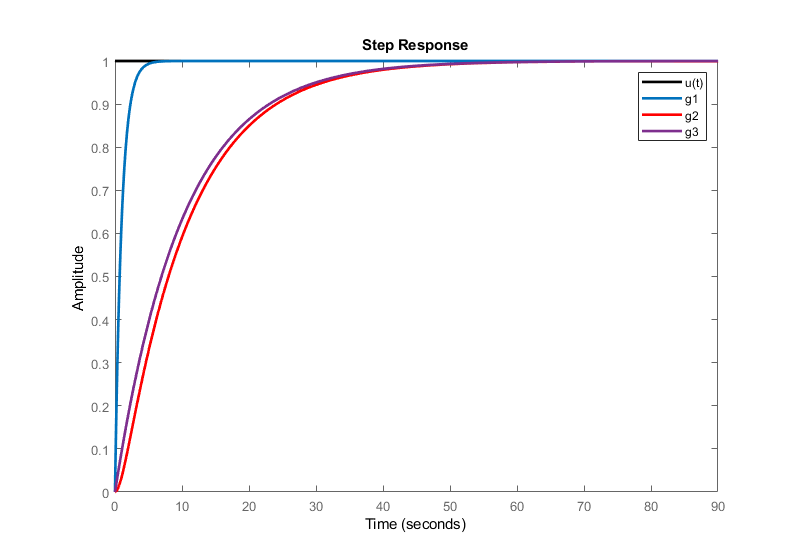
\includegraphics[width=1.0\unitlength]{q3a}
		\caption{\label{fig:q3}Step Responses of Bare($G_1$) and Sheath($G_2$) Thermocouples }
	\end{figure}
	
	\item It stated that that the time constant of the bare thermocouple is usually much smaller than the one caused by sheathing. Therefore, one may approximate the overall transfer function as a first order one as can be interpreted from the \textit{Figure~\ref{fig:q3}}.
	
	$$ G(s)=\frac{K}{1+\tau_2 s} $$
	
	It is also given that, the voltage generated across wires would be
	
	$$ V(t)= \Delta V\left( 1-e^{-\cfrac{t}{\tau_2}}\right)+V_0$$ 
	$$ V(\tau_2)= \Delta V\left( 1-e^{-\cfrac{\tau_2}{\tau_2}}\right)+V_0=\Delta V\left( 1-e^{-1}\right)+V_0$$ 
	$$\boxed{ V(\tau_2)= 0.632\Delta V+V_0}$$
	
	$$ ln \left(1-\frac{V(t)-V_0}{\Delta V} \right)=-\frac{t}{\tau_2}$$
	
	$$\boxed{ \tau_2=\cfrac{-t}{ln \left(1-\cfrac{V(t)-V_0}{\Delta V} \right)}}$$

	\item Pole-Zero plot for the bare($G_1$) and sheath($G_2$) thermocouple models can be seen at \textit{Figure~\ref{fig:q5}}
	
	\begin{figure}[H]
		\center
		\setlength{\unitlength}{\textwidth} 
		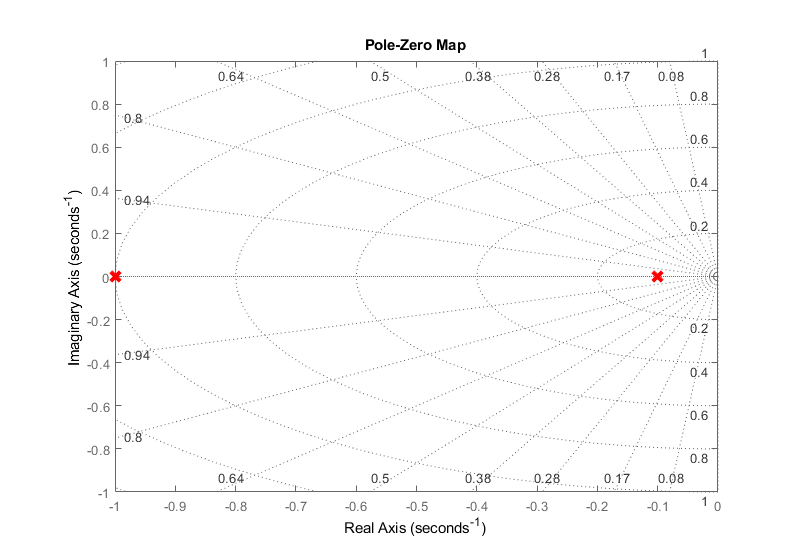
\includegraphics[width=1.0\unitlength]{q4}
		\caption{\label{fig:q5}Pole-Zero plot for the Bare($G_1$) and Sheath($G_2$) Thermocouple Models }
	\end{figure}
	
	\item 
	
		$$ v_i=v_c+v_o$$
		$$ v_c=v_i-v_o$$
		$$ i_c+i_{R_1}=i_{R_2}$$
		$$ I_c(s)=sCV_c(S)=sC(V_c(s))=\frac{V_o(s)}{R_2}-\frac{V_c(s)}{R_1}$$	
		$$ \left( sC+\frac{1}{R_1}\right) [Vi(s)-V_o(s)]=\frac{V_0}{R_2}$$
		$$ \vdots$$
		$$ G(s)=\frac{V_o(s)}{V_i(s)}=\frac{sCR_1R_2+R_2}{sCR_1R_2+R_1+R_2}=\alpha\frac{1+\tau_c s }{1+ \alpha \tau_c s}$$
		Thus,
		$$ \boxed{\alpha = \frac{R_2}{R_1+R_2}} \ , \ \boxed{\tau_c=cR_1}$$
		It can be seen from the above equation that $0<\alpha<1$ according to resistor values. Therefore, it can be concluded that the compensator is indeed a \textbf{Lead Compensator}.
		
		\item With $\alpha=0.5$ and $\tau_c=\tau_2=10\ seconds$
		
		$$ G_{ovll}(s)=\frac{1}{(10s+1)}\frac{1+10s}{2(1+5s)}$$
		
		The step response of overall system can be seen at \textit{Figure~\ref{fig:q6}}.
		
		\begin{figure}[H]
			\center
			\setlength{\unitlength}{\textwidth} 
			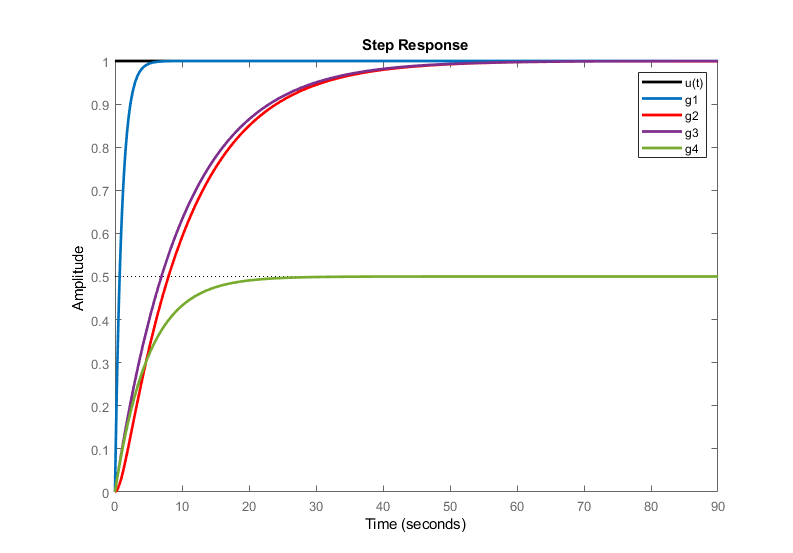
\includegraphics[width=1.0\unitlength]{q6}
			\caption{\label{fig:q6}Step Responses of Bare($G_1$) and Sheath($G_2$) Thermocouples and Sheath Thermocouple with Compensator($G_4$}
		\end{figure}
		
		\item With $\tau_c=12\ seconds$
		
		$$ G_{5}(s)=\frac{1}{(10s+1)}\frac{1+12s}{2(1+6s)}$$
				
				With $\tau_c=8\ seconds$
		
		$$ G_{6}(s)=\frac{1}{(10s+1)}\frac{1+8s}{2(1+4s)}$$
		
		The step responses were exactly the same for the plot limits of MATLAB, the response can be seen at \textit{Figure~\ref{fig:q8}}.
				
		\begin{figure}[H]
			\center
			\setlength{\unitlength}{\textwidth} 
			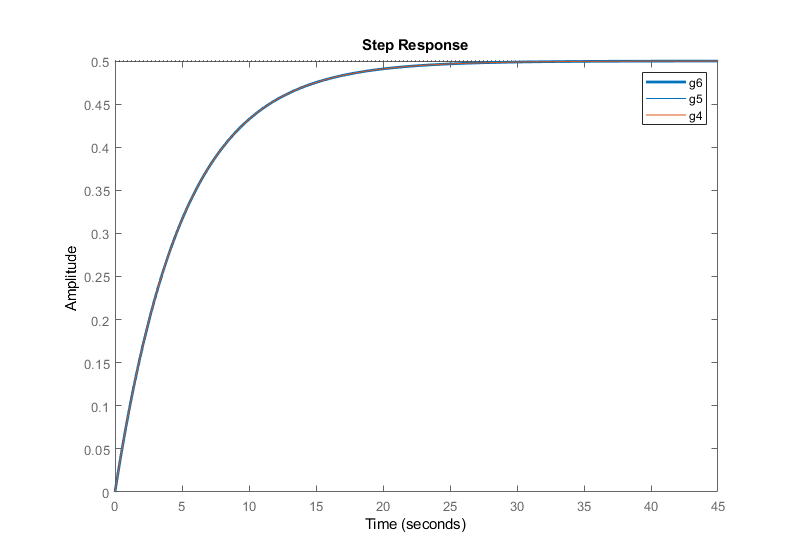
\includegraphics[width=1.0\unitlength]{q8}
			\caption{\label{fig:q8}Step Responses of Sheath Thermocouple with Compensator Parameters($G_4$}
		\end{figure}
		
	
\end{enumerate}
	
\begin{appendices}
\section{Source Code for Matlab Part}\label{appendix}
	%%	\lstinputlisting[language=Matlab,firstline=33, lastline=34]{q13.m} \-\\[1cm]		
\lstinputlisting[language=Matlab]{EXP1.m} 
\end{appendices}

\end{document}

%----samples------
%\begin{itemize}
%\item Item
%\item Item
%\end{itemize}

%\begin{figure}[H]
%\center
%\setlength{\unitlength}{\textwidth} 
%\includegraphics[width=0.7\unitlength]{images/logo1}
%\caption{\label{fig:logo}Logo }
%\end{figure}

%\begin{figure}[H]
%	\setlength{\unitlength}{\textwidth} 
%	\centering
%	\begin{subfigure}{.5\textwidth}
%  		\centering
%  		\includegraphics[width=0.48\unitlength]{images/logo1}
%  		\caption{\label{fig:logo1}Logo1 }
%	\end{subfigure}%
%	\begin{subfigure}{.5\textwidth}
%  		\centering
%		\includegraphics[width=0.48\unitlength]{images/logo2}
%  		\caption{\label{fig:logo2}Logo2}
%	\end{subfigure}
%\caption{\label{fig:calisandegree} Small Logos   }
%\end{figure}
	
%\begin{table}[H]
%  \centering
% 
%    \begin{tabular}{c|c|c}
%       $$A$$ & $$B$$ & $$C$$ \\ \hline
%       1 & 2 & 3  \\ \hline
%       2 & 3 & 4  \\ \hline
%       3 & 4 & 5  \\ \hline
%       4 & 5 & 6  
%      
%  \end{tabular}
%  \caption{table}
%  \label{tab:table}
%\end{table}
	
%\begin{table}[H]
%  \centering
% 
%    \begin{tabular}{c|c|c}
%       \backslashbox{$A$}{$a$} & $$\specialcell{ Average deviation \\ after subtracting out the  \\ frequency error }$$ & $$C$$ \\ \hline
%       \multirow{2}{*}{1} & 2 & 3  \\ \cline{2-3}
%        & 3 & 4  \\ \hline
%       3 & \multicolumn{2}{c}{4}  \\ \hline
%       4 & 5 & 6  
%      
%  \end{tabular}
%  \caption{table}
%  \label{tab:table}
%\end{table}
%-----end of samples-----